% Buck Converter
% Topology: Vin -> IGBT switch -> freewheeling diode -> L -> C || R_L -> Vout

\documentclass[border=5pt]{standalone}
\usepackage{tikz}
\usepackage[american,cuteinductors,smartlabels]{circuitikz}

% Component dimensions
\ctikzset{bipoles/thickness=0.7}
\ctikzset{bipoles/length=1.5cm}
\ctikzset{bipoles/resistor/width=0.7}
\ctikzset{bipoles/resistor/height=0.25}
\ctikzset{bipoles/diode/height=0.3}
\ctikzset{bipoles/diode/width=0.3}
\ctikzset{tripoles/thickness=0.7}
\ctikzset{bipoles/battery1/height=0.7}

% Global styles
\tikzstyle{every node}=[font=\Large]
\tikzstyle{every path}=[line width=0.9pt, line cap=round, line join=round]

\begin{document}
\begin{circuitikz}

  % --- Coordinate origin ---
  \coordinate (VBottom) at (0,0);

  % --- Input voltage source (+ at top) ---
  \draw (VBottom) to[battery1, l=$V_{in}$, invert] ++(0,3) coordinate (VTop);

  % --- IGBT switch (horizontal, drain anchored to VTop rail) ---
  \draw (VTop) to[short] ++(0.8,0)
    node[nigbt, anchor=C, rotate=90,
         label={[yshift=-1.5cm] \normalsize $Q_1$}] (Q1) {};

  % --- From IGBT emitter: create SW node, then inductor ---
  \draw (Q1.E) to[short] ++(0.5,0) coordinate (SwNode)
    to[short] ++(0.5,0)
    to[L, l_=$L$, v^=$v_L$, i>_=$i_L$] ++(2.5,0) coordinate (InductorRight);

  % --- Freewheeling diode: from SW node down to ground rail ---
  \draw (SwNode) to[D*, invert] (SwNode|-VBottom);

  % --- Output capacitor ---
  \draw (InductorRight) to[short] ++(0.5,0) coordinate (CapTop)
    to[C, l_=$C$, i>^=$i_C$] (CapTop|-VBottom);

  % --- Load resistor + output voltage label ---
  \draw (CapTop) to[short] ++(1.5,0) coordinate (ResTop)
    to[R, l_=$R_L$, v^=$V_{out}$] (ResTop|-VBottom) coordinate (ResBottom);

  % --- Ground rail ---
  \draw (ResBottom) -- (VBottom);

  % --- Gate drive signal ---
  \draw (Q1.B) -- ++(0,0.8) node[above] {$g$};

\end{circuitikz}

%------ Conversion Ratio
\begin{tikzpicture}
  \coordinate[label={[xshift=0,yshift=0]
    \large $M(D)=\dfrac{V_{out}}{V_{in}}=D; \quad 0 \leq D \leq 1$}]
    (M) at (3,0);
\end{tikzpicture}

\end{document}
